\documentclass[11pt,a4paper]{article}
\usepackage[utf8]{inputenc}
\usepackage[margin=0.75in]{geometry}
\usepackage{graphicx}
\usepackage{xcolor}
\usepackage{hyperref}
\usepackage{titlesec}
\usepackage{enumitem}
\usepackage{tcolorbox}
\usepackage{booktabs}
\usepackage{caption}
\usepackage{microtype} % Better line breaking to save space

% Custom Colors
\definecolor{primary}{HTML}{1A237E}
\definecolor{highlight}{HTML}{7E57C2}
\definecolor{logic}{HTML}{00897B}
\definecolor{action}{HTML}{F57C00}

\titleformat{\section}{\large\bfseries\color{primary}}{}{0em}{}[\titlerule]
\titleformat{\subsection}{\normalsize\bfseries\color{highlight}}{}{0em}{}
\titlespacing*{\section}{0pt}{1.5ex plus 1ex minus .2ex}{0.8ex plus .2ex}
\titlespacing*{\subsection}{0pt}{1.2ex plus 1ex minus .2ex}{0.5ex plus .2ex}

\title{\Huge \textbf{FinMentor AI \& ArthaScan} \\ \Large A Unified Architecture for Zero-Hallucination Financial Advice}
\author{\textbf{Hackathon Submission: PS 9 - AI Money Mentor}}
\date{\today}

\begin{document}

\maketitle
\vspace{-4em} % Push content upwards

\begin{tcolorbox}[colback=blue!5!white,colframe=blue!75!black,title=Executive Summary,boxsep=1pt,left=2pt,right=2pt,top=2pt,bottom=2pt]
\small The FinMentor AI ecosystem addresses the critical problem of automated financial advice: \textbf{Trust vs. Generative Noise}. Our architecture implements a "Zero-Hallucination" philosophy by strictly isolating all mathematical and business logic from the Large Language Models (LLMs). The LLMs are utilized solely for multi-channel data extraction and conversational translation, while 100\% of the financial truths are derived from deterministic Python engines.
\end{tcolorbox}

\section{System Architecture Overview}
The system enables a dual-channel experience via a full \textbf{React Web Dashboard} and a frictionless \textbf{Telegram Bot Interface}. Both channels converge on a unified high-resolution extraction and analysis pipeline.

\begin{center}
    \vspace{-1em}
    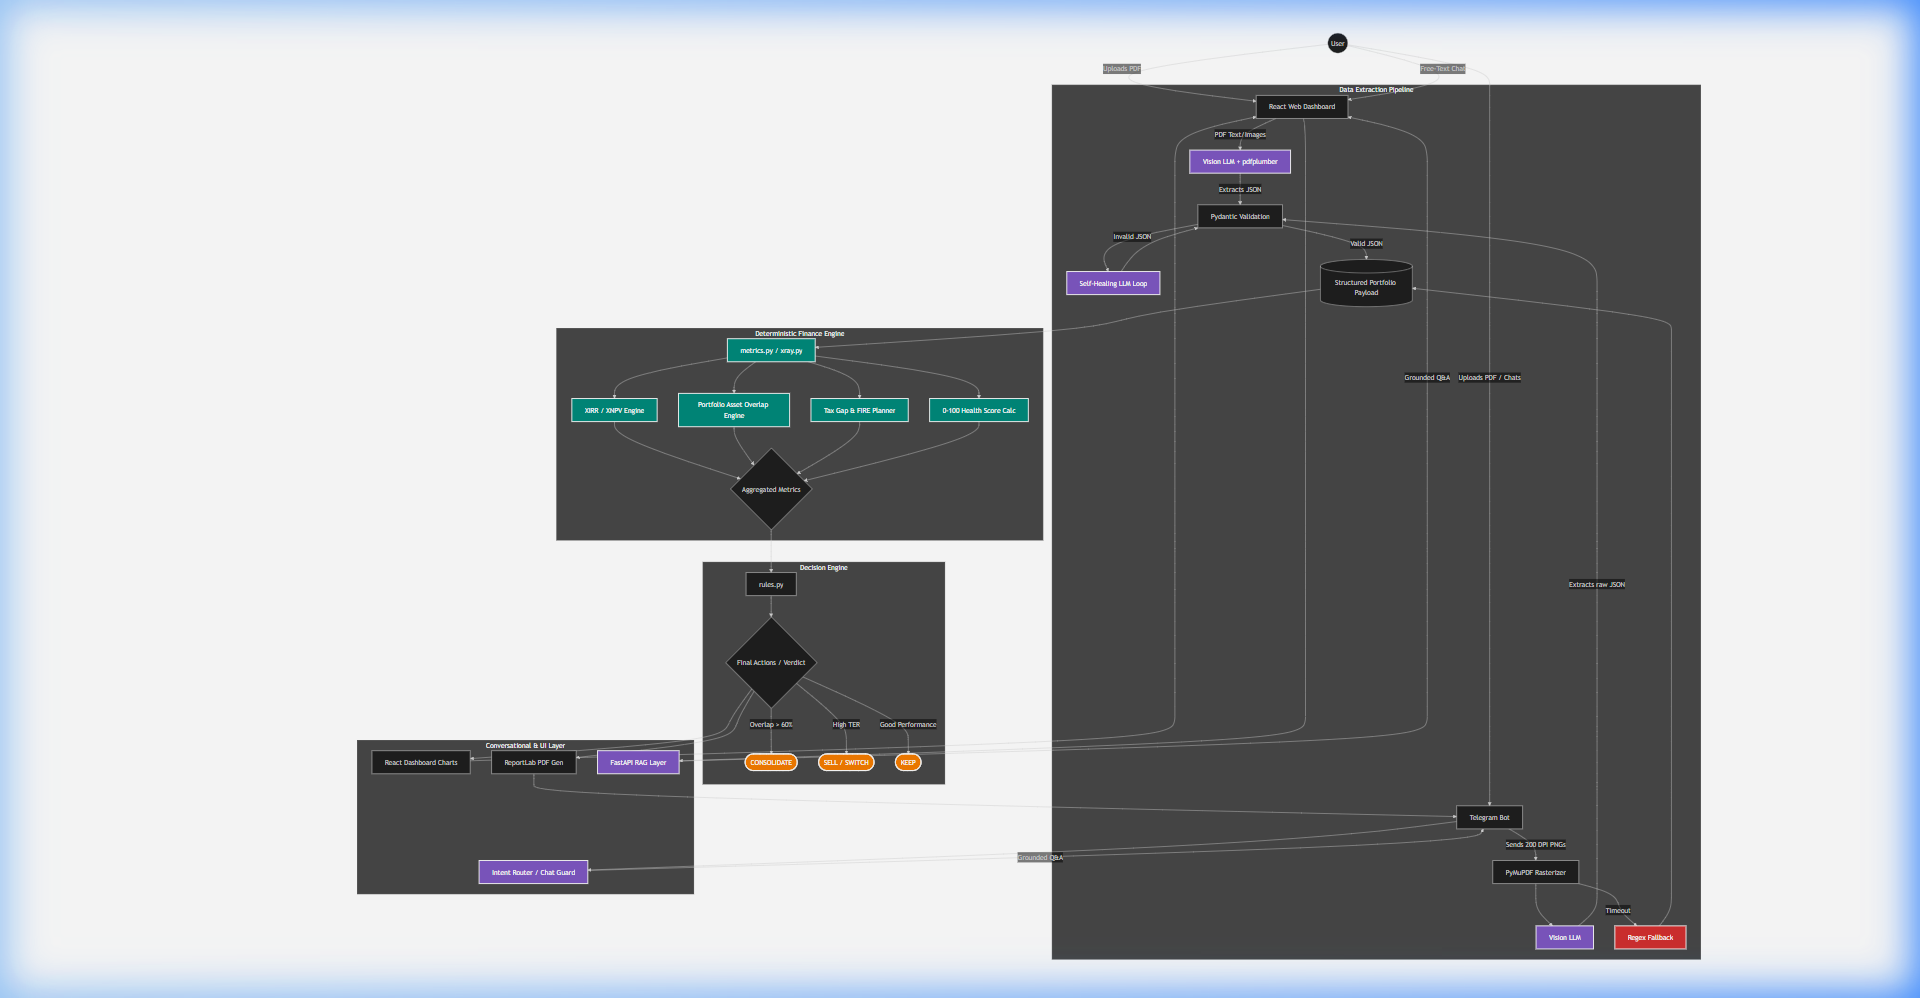
\includegraphics[width=0.95\textwidth]{architecture.png}
    \captionof{figure}{\small High-Level System Flow: Extraction, Calculation, and Decision Layers}
    \vspace{-1.5em}
\end{center}

\section{I. Multimodal Data Extraction Pipeline}
Large Language Models often struggle with dense, tabular financial statements (CAMS/KFintech). Our pipeline bypasses traditional text-crawling vulnerabilities through a Vision-First approach:

\begin{itemize}[leftmargin=*,nosep]
    \item \textbf{Image Rasterization/Vision:} Documents are converted to 200 DPI PNGs via `PyMuPDF` to avoid character mangling, then parsed by Vision LLMs into typed JSON.
    \item \textbf{Self-Healing Loop:} Validated via Pydantic; if malformed, the system recursively prompts for syntax repairs before analysis.
    \item \textbf{Regex Fallback:} A silent parser acts as a safety net during API timeouts, ensuring data stability.
\end{itemize}

\section{II. The Deterministic Financial Engine}
In our architecture, the AI is "Math-Blind." Once the data is extracted, it enters a walled-off sandbox where only pure Python algorithms are permitted to operate.

\subsection{1. The XIRR Computing Engine}
Instead of relying on LLM estimations, we implement a binary-search algorithm performing standard \textbf{XNPV} calculations against exact historical cashflows. This ensures the reported XNPV and XIRR are 100\% audited and mathematically sound.

\subsection{2. Portfolio Overlap \& Duplication}
The engine normalizes individual stock exposures across all mutual funds. By calculating the intersection of thousands of underlying assets, the system identifies hidden portfolio duplication—often revealing that users are paying multiple management fees for the same underlying stocks.

\subsection{3. Wealth Bleed Analysis}
The engine calculates the "Visible vs. Invisible Cost" by compounding the user's specific Expense Ratio (TER) against a Direct Plan baseline (0.1--0.5\%) over a 10-year horizon.

\section{III. Rigid Rules-Based Decision Hierarchy}
The transition from "Math" to "Advice" is governed by a hardcoded heuristic tree (\texttt{rules.py}). The system categorizes each fund based on specific financial thresholds:

\begin{table}[h!]
\centering
\small
\setlength{\tabcolsep}{4pt}
\begin{tabular}{ll}
\toprule
\textbf{Condition} & \textbf{System Directive} \\
\midrule
Asset Overlap $> 60\%$ & \textbf{CONSOLIDATE} (Instructions to merge folios) \\
Expense Drag $> 1.0\%$ & \textbf{SWITCH} (Transition from Regular to Direct) \\
Closet Index Tracking & \textbf{SELL} (Moving to low-cost Index alternatives) \\
Underperformance vs Peer & \textbf{REVIEW} (Watchlist placement) \\
\bottomrule
\end{tabular}
\end{table}
\vspace{-1ex}

\section{IV. "Glass-Box" Presentation \& Intent Routing}
The AI layer (Agent) serves as the presentation face. An \textbf{Intent Router} ensures that conversational queries are always grounded:
\begin{itemize}[nosep]
    \item \textbf{Math Queries:} Pure numerical requests bypass the LLM and pull from the Math Engine.
    \item \textbf{Explanation Agent:} The LLM translates deterministic JSON facts into English/Hinglish without hallucinating new data.
\end{itemize}

\section{Technology Stack}
\begin{itemize}[nosep]
    \item \textbf{Core Engine:} Python 3.11+, pyxirr, NumPy, Pydantic.
    \item \textbf{Backend/Frontend:} FastAPI, Telegram Bot API, React 18, Recharts.
\end{itemize}

\end{document}
